\begin{frame}{The Margin Is Uncertain}

\begin{columns}[c,onlytextwidth]

\column{0.52\textwidth}
\centering
\resizebox{\linewidth}{!}{%
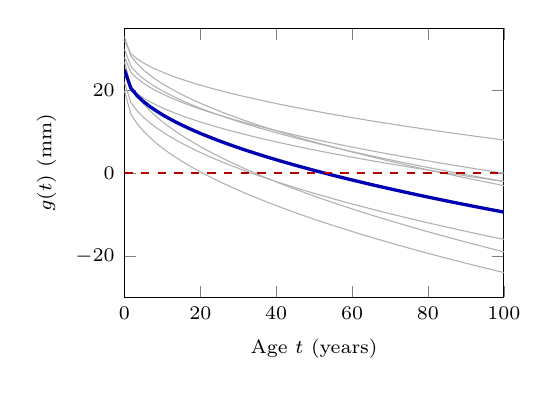
\begin{tikzpicture}
\begin{axis}[
  width=6.4cm, height=5.0cm,
  xlabel={Age $t$ (years)}, ylabel={$g(t)$ (mm)},
  xmin=0, xmax=100, ymin=-30, ymax=35,
  label style={font=\scriptsize}, tick label style={font=\scriptsize},
]
  \addplot[domain=0:100, samples=60, gray!60, thin] {32 - 2.4*sqrt(x)};
  \addplot[domain=0:100, samples=60, gray!60, thin] {28 - 2.8*sqrt(x)};
  \addplot[domain=0:100, samples=60, gray!60, thin] {22 - 3.8*sqrt(x)};
  \addplot[domain=0:100, samples=60, gray!60, thin] {30 - 3.2*sqrt(x)};
  \addplot[domain=0:100, samples=60, gray!60, thin] {20 - 4.4*sqrt(x)};
  \addplot[domain=0:100, samples=60, gray!60, thin] {27 - 4.6*sqrt(x)};
  \addplot[domain=0:100, samples=60, gray!60, thin] {24 - 2.6*sqrt(x)};
  \addplot[domain=0:100, samples=60, gray!60, thin] {33 - 3.6*sqrt(x)};
  \addplot[domain=0:100, samples=60, blue!70!black, very thick] {25 - 3.44*sqrt(x)};
  \addplot[red!70!black, thick, dashed] coordinates {(0,0) (100,0)};
\end{axis}
\end{tikzpicture}%
}

{\scriptsize Illustrative trajectories.}

\column{0.44\textwidth}
\justifying
Concrete strength, humidity, cover and CO$_2$ are uncertain, so each element follows a different trajectory.

\vspace{0.3cm}

\begin{exampleblock}{Probability of depassivation}
\[
  P_f(t) = P\left[g(t) \le 0\right]
\]
\end{exampleblock}

\vspace{0.2cm}

{\small Example (25 MPa, 25 mm cover): without maintenance, $P_f(100) \approx 0.88$.}

\end{columns}

\end{frame}
